\section{Lasermoden}
\subsection{Darstellung verschiedener transversaler Moden}
Die transversalen Moden wurden in unserem Versuch zum Schluss aufgenommen. Dies hat 
den einfachen Grund, dass die transversalen Moden durch die falsche Justierung sichtbar
gemacht werden können. Wir haben die transversalen Moden gefunden, indem 
wir bewusst die Spiegel verstellt haben und zusätzlich ein Drahtgitter in den Strahlengang eingebaut haben.\\ 
Die Moden werden dann durch 
eine Linse vergrößert und auf eine Wand projiziert, um diese besser erkennen zu können.
Anschließend wird ein Bild von der Mode mithilfe eines Smartphones aufgenommen. \\
Die gefundenen Moden sind im Folgenden zu sehen: 
\begin{figure}[h]
    \centering
    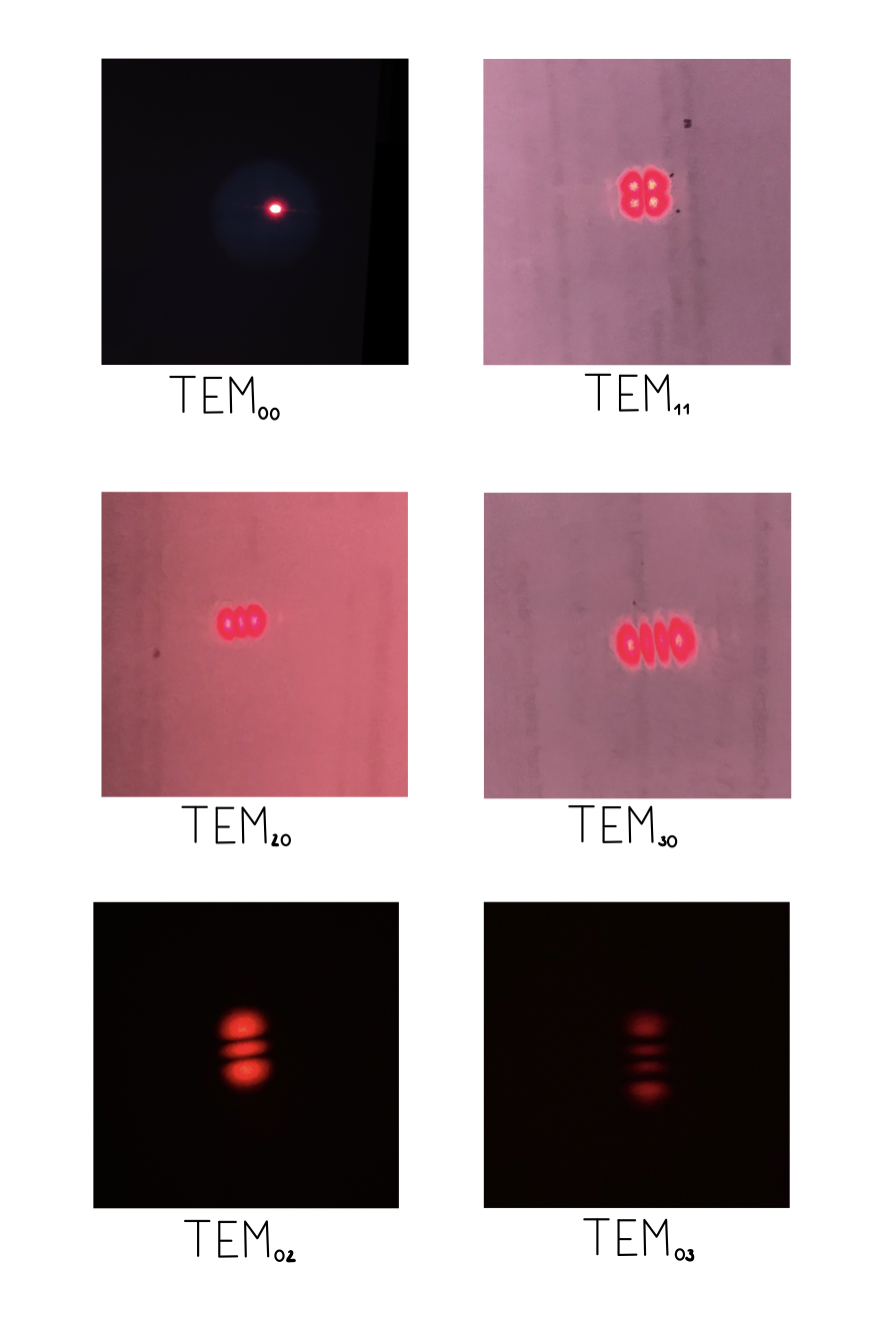
\includegraphics[scale=0.28]{Bilder/Auswertung Anna/TEM.jpg}
    \caption{Aufnahmen der verschiedenen transversalen Moden.}
   \end{figure}
\newpage
Die Benennung erfolgte mithilfe der in der Theorie gezeigtem Bild \ref{fig:Tmode}.\\
Auf den Bildern ist es leider schwer zu erkennen, aber die Grundmode ($\text{TEM}_{00}$) 
war die stabilste und die mit der höchsten Intensität, was auch nicht weiter überraschend ist. 
Die höheren Mode wurden immer instabiler und 'verschwommener'. Die Moden die aufgenommen wurden 
waren die identifizierbaren, es kam während dem Versuch aber auch immer wieder zu Mischformen zwischen
den verschiedenen Moden. 
